\section{\texorpdfstring{$\mathcal{H}_\infty$} Design}\label{sec:Hinf}
The linearized model in \autoref{sec:linearizationModel} has varying parameters, such as the added mass and damping coefficients. The vessel may also experience external disturbances, such as wind forces. During surveying, the vessel needs to be robust to these model variations and it must be able to sufficiently reject disturbances. Using the $\mathcal{H}_\infty$ design technique, a robust controller for the vessel can be synthesized. The design of such controller differs from the LQR design. In this case, the design of model and controller is done simultaneously and can not be clearly separated as for the LQR case.

The $\mathcal{H}_\infty$ problem consists of finding an internally stabilizing controller that provides a closed loop $\mathcal{H}_\infty$ norm less than some bound $\gamma$ \cite[p. 835]{JCDoyle}, \cite[pp. 92-93]{AAStoorvogel}. Such controller is also called suboptimal $\mathcal{H}_\infty$ controller, as there might be smaller $\gamma$ yielding an internally stabilizing controller.% The reason for not deigning the optimal controller is \fxnote{write reason}

A more detailed mathematical formulation of the $\mathcal{H}_\infty$ problem and its solution is given in \cite[pp. 91-119]{AAStoorvogel}. 

The state space model from \autoref{xDotLinear} and \autoref{yLinear} needs to be remodeled into a state space form suitable for solving the suboptimal $\mathcal{H}_\infty$ control problem. This representation starts with the equations
For solving the suboptimal $\mathcal{H}_\infty$ control problem, the system has to be expressed in a particular state space form \cite[pp. 95]{AAStoorvogel}, \cite[p. 64]{robustNotes}. This form is
\begin{flalign}
  \vec{\dot{x}}(t) &= \vec{A}_1 \vec{x}(t) + \vec{B}_1 \vec{w}(t) + \vec{B}_2 \vec{u}(t)\ ,
  \label{eq:xDotHinf} \\
  \vec{z}(t) &= \vec{C}_1 \vec{x}(t) + \vec{D}_{11} \vec{w}(t) + \vec{D}_{12} \vec{u}(t)\ ,
  \label{eq:zHinf} \\
  \vec{y}(t) &= \vec{C}_2 \vec{x}(t) + \vec{D}_{21} \vec{w}(t) + \vec{D}_{22} \vec{u}(t)\ ,
  \label{eq:yHinf} 
\end{flalign}
\begin{where}
  \va{\vec{x}}{is the state vector}{}
  \va{\vec{w}}{is the uncontrolled input vector}{}
  \va{\vec{u}}{is the controlled input vector}{}
  \va{\vec{z}}{is the performance output vector}{}
  \va{\vec{y}}{is the measured output vector}{}
  \va{\vec{A}_1}{is the state matrix}{}
  \va{\vec{B}_1}{is the uncontrolled input matrix}{}
  \va{\vec{B}_2}{is the controlled input matrix}{}
  \va{\vec{C}_1}{is the performance output matrix}{}
  \va{\vec{D}_{11}}{is the direct feedthrough matrix from $\vec{w}$ to $\vec{z}$}{}
  \va{\vec{D}_{12}}{is the direct feedthrough matrix from $\vec{u}$ to $\vec{z}$}{}
  \va{\vec{C}_2}{is the measured output matrix}{}
  \va{\vec{D}_{21}}{is the direct feedthrough matrix from $\vec{w}$ to $\vec{y}$}{}
  \va{\vec{D}_{22}}{is the direct feedthrough matrix from $\vec{u}$ to $\vec{y}$}{}
\end{where}

The $\mathcal{H}_\infty$ model representation can also be seen in \autoref{fig:HinfDiag}, where all signals and matrices involved in the design process are represented.
\begin{figure}[H]
	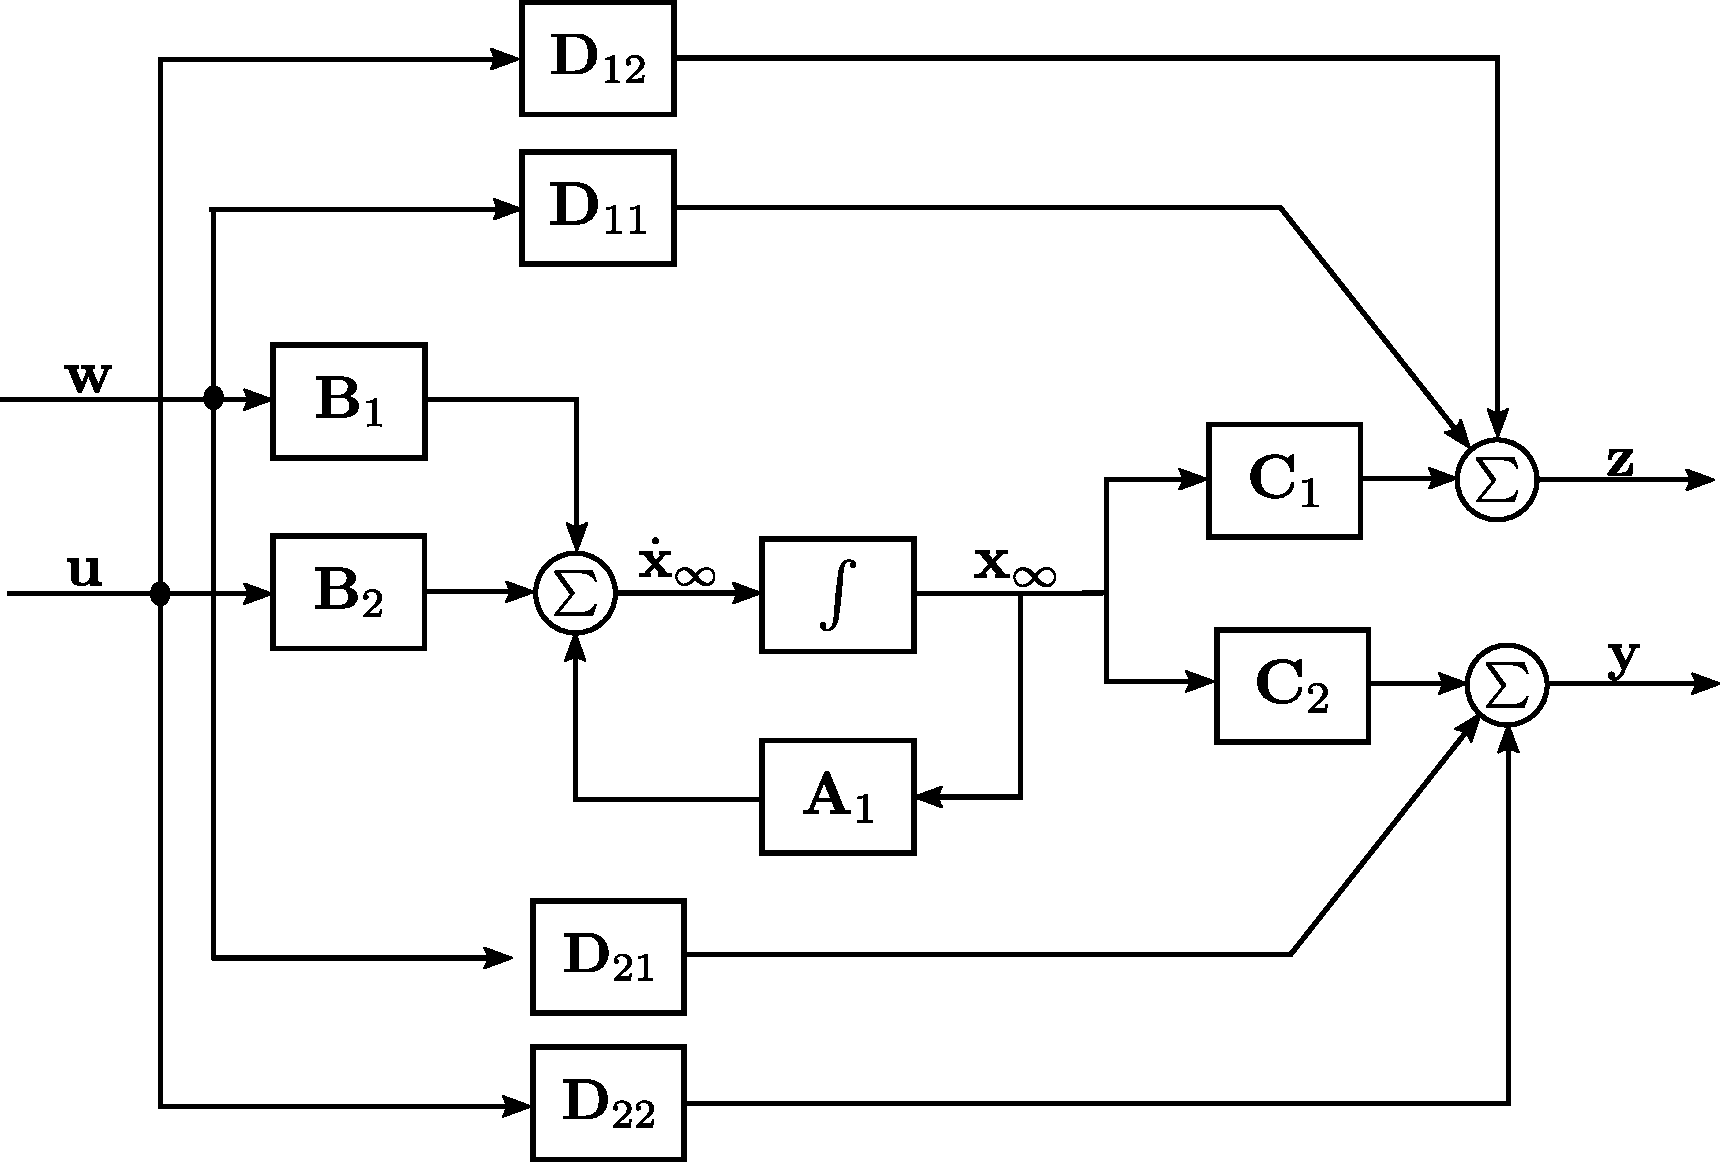
\includegraphics[width=0.6\textwidth]{figures/HinfDiag}
	\caption{Block diagram used in the $\mathcal{H}_\infty$ controller design.}
	\label{fig:HinfDiag}
\end{figure}

The method used to achieve the solution to the problem requires assuming certain conditions on the matrix in the model \cite[p. 835]{JCDoyle}. These conditions are 
\begin{itemize}
	\item $\left (\vec{A}_1,\vec{B}_1 \right)$ and $\left( \vec{A}_1, \vec{B}_2 \right)$ are stabilizable.
	\item $\left (\vec{C}_1,\vec{A}_1 \right)$ and $\left( \vec{C}_2, \vec{A}_1 \right)$ are detectable.
	\item $\vec{D}_{12}^\mathrm{T}[\vec{C}_1\ \vec{D_{12}}]$ is $[\vec{0}\ \vec{I}]$.
	\item $\begin{bmatrix}
				\vec{B}_1 \\
				\vec{D}_{21} 
			\end{bmatrix}\vec{D}_{21}^\mathrm{T}$ is $[\vec{0}\ \vec{I}]$.
	\item $\vec{D}_{11}$ and $\vec{D}_{22}$ are zero.
\end{itemize}

For obtaining the matrices present in \autoref{eq:xDotHinf}, \ref{eq:zHinf} and \ref{eq:yHinf}, the content of the state vector and signal vectors needs to be defined.

\subsection*{State Vector}
The state vector construction starts with the three states that define the basic dynamics of the system. Namely, $\psi$, $\dot{\psi}$ and $\dot{x}_\mathrm{b}$. As some reference tracking is desired, integral states need to be included in the state vector, these depend on the measured output and the reference signal as 
\begin{flalign}
	\vec{\dot{x}}_\mathrm{int} =
	\begin{bmatrix}
		x_{int_{\psi}} \\
		x_{int_{\dot{x}_\mathrm{b}}}
	\end{bmatrix}\ = 
	\begin{bmatrix}
		\psi_\mathrm{ref}-\psi \\
		\dot{x}_\mathrm{b,ref} - \dot{x}_\mathrm{b}
	\end{bmatrix}\ .
	\label{eq:xintVectorHinf}
\end{flalign}

The state vector also includes the states coming from the reference, disturbance and noise models. These extra states, not only show the dynamics of the uncontrolled inputs, but also reflect the weighting functions that have been applied to each of them. This process is carried out in order to modify how the uncontrolled inputs affect the states, this is normally done through transfer functions, \cite{MSalari}. In order to include weights in the state space representation, some states for each uncontrolled input need to be defined. \autoref{fig:WeightDiag} shows an example of how an uncontrolled input is weighted so it can be included in the state space representation.
\begin{figure}[H]
	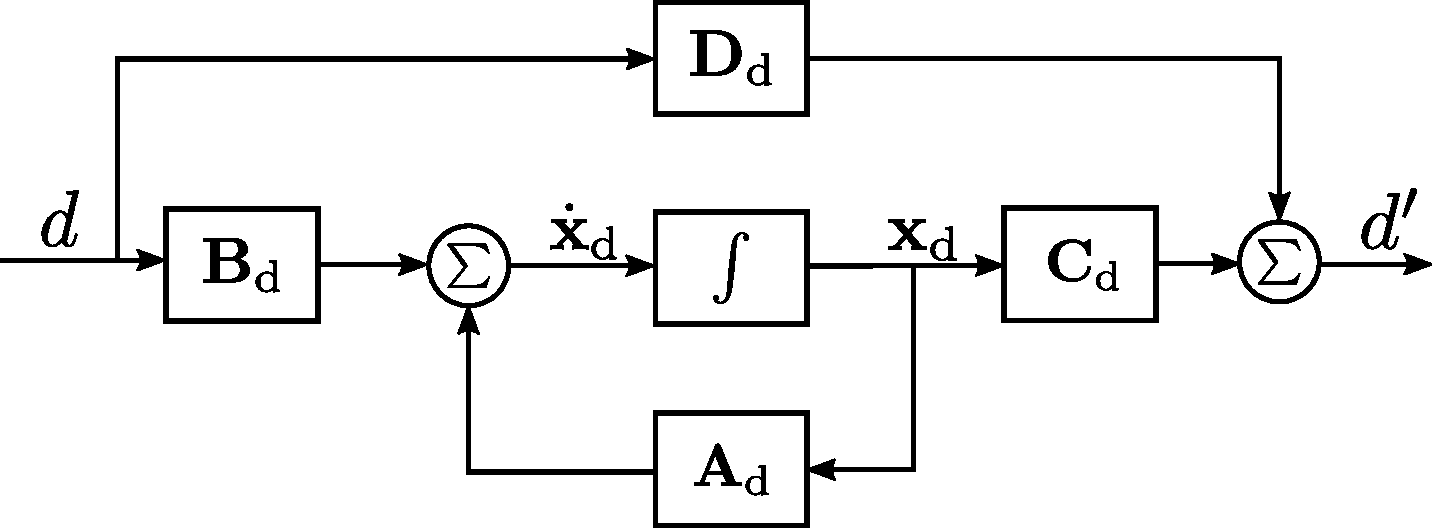
\includegraphics[width=0.6\textwidth]{figures/WeightDiag}
	\caption{Block diagram illustrating how an uncontrolled input is weighted in the $\mathcal{H}_\infty$ controller design. $d$ is the uncontrolled input and $d'$ is the weighted uncontrolled input. The states $\vec{x}_\mathrm{d}$ are included in the state vector of the $\mathcal{H}_\infty$ state space representation.}
	\label{fig:WeightDiag}
\end{figure}
The uncontrolled input states are part of the state vector. The $\vec{A}_\mathrm{d}$, $\vec{B}_\mathrm{d}$, $\vec{C}_\mathrm{d}$ and $\vec{D}_\mathrm{d}$ in \autoref{fig:WeightDiag} can be calculated from a weighting function as in the example given in \autoref{eq:weightingexampleLP}, where the uncontrolled input $d$ is weighted by means of a first order transfer function with low-pass characteristics.
\begin{flalign}
	\frac{d'}{d}=\frac{a}{s+a} \rightarrow \dot{d}' = -a d' + a d \rightarrow \begin{cases} \dot{x}_\mathrm{d} = -a x_\mathrm{d} + a d \\ d' = x_\mathrm{d} \end{cases}\label{eq:weightingexampleLP} 
\end{flalign}
\begin{where}
	\va{a}{is a parameter defining the pole position of the weighting function}{}
\end{where}
Another example with a high pass weighting function is shown in \autoref{eq:weightingexampleHP}.
\begin{flalign}
	\frac{n'}{n}=\frac{s}{s+a} = \frac{-a}{s+a}-1 \rightarrow \begin{cases} \dot{x}_\mathrm{n} = -a x_\mathrm{n} + n \\ n' = - a x_\mathrm{n} + n  \end{cases}\label{eq:weightingexampleHP} 
\end{flalign}

This process also entails defining the weights for each uncontrolled input. The weight on the reference is set to be a first order transfer function with a very fast pole so the step input does not get distorted. The weights on the input disturbances are also low pass filtered as most of them appear at low frequencies. The noise, on the other hand, is weighted according to a high pass filter, as it is stronger in the high frequency range. In this way, the controller design focuses on achieving a robust controller with respect to the uncontrolled inputs in their particular frequency ranges. The chosen frequencies are 1, 20 and 20 rad/s for the references, wind disturbance and wave disturbance low pass filters, respectively, and 100 rad/s for the noise high pass filter. These numbers are calculated based on several test which can be seen in \fxnote{make appendix with freq tests} The weights for each uncontrolled input are

\hspace{0.2\linewidth}
\begin{minipage}{0.3\linewidth}
\begin{flalign}
	W_{\psi_\mathrm{ref}} &= \frac{1}{s+1}\ ,\nonumber \\
	W_{F_\mathrm{wind}} &= \frac{20}{s+20}\ ,\nonumber\\
	W_{F_\mathrm{wave}} &= \frac{20}{s+20}\ ,\nonumber\\
	W_{n_\psi} &= \frac{s}{s+100}\ .\nonumber
\end{flalign}
\end{minipage}
\begin{minipage}{0.3\linewidth}
\begin{flalign}
	W_{\dot{x}_\mathrm{b,ref}} &= \frac{1}{s+1}\ ,\nonumber \\
	W_{\tau_\mathrm{wind}} &= \frac{20}{s+20}\ , \nonumber\\
	W_{\tau_\mathrm{wave}} &= \frac{20}{s+20}\ , \nonumber\\
	W_{n_{\dot{x}_\mathrm{b}}} &= \frac{s}{s+100}\ .\nonumber
\end{flalign}
\end{minipage}\hfill
%\begin{flalign}
%	W_{\psi_\mathrm{ref}} = \frac{1}{s+1}\ ,\  W_{\dot{x}_\mathrm{b,ref}} = \frac{1}{s+1}\ ,\nonumber \\
%	W_{F_\mathrm{wind}} = \frac{1}{s+1}\ ,\nonumber\   W_{\tau_\mathrm{wind}} = \frac{1}{s+1}\ , \nonumber\\
%	W_{F_\mathrm{wave}} = \frac{1}{s+1}\ , \nonumber\  W_{\tau_\mathrm{wave}} = \frac{1}{s+1}\ , \nonumber\\
%	W_{n_\psi} = \frac{s}{s+1}\ , \nonumber\ 	W_{n_{\dot{x}_\mathrm{b}}} = \frac{s}{s+1}\ .\nonumber
%\end{flalign}

The states coming from the weighting functions, together with the system states and the integral states, constitute the state vector as 
\begin{flalign}
	\vec{x}(t)=
	\begin{bmatrix}
		\psi & \dot{\psi} & \dot{x}_\mathrm{b} & x_{int_{\psi}} & x_{int_{\dot{x}_\mathrm{b}}} & x_{F_\mathrm{wind}} & x_{\tau_\mathrm{wind}} & x_{F_\mathrm{wave}} & x_{\tau_\mathrm{wave}} & x_{n_{\psi}}\ \ \  x_{n_{\dot{x}_\mathrm{b}}}
	\end{bmatrix}^\mathrm{T}\ .
	\label{eq:xVectorHinf}
\end{flalign}

\subsection*{Controlled Inputs Vector}
The controlled input are the two forces provided by the thrusters of the boat, that is, 
\begin{flalign}
	\vec{u(t)}= 
	\begin{bmatrix}
		F_1 & F_2 
	\end{bmatrix}^\mathrm{T}\ .
	\label{eq:uVectorHinf}
\end{flalign} \nonumber


\subsection*{Uncontrolled Input vector}
The uncontrolled inputs include the references to be tracked, the input disturbances, and the measurement noises. The size of this vector depends on the amount of reference signals, the input disturbances considered (wind, waves) and the amount of measured outputs, as these are normally affected by noise. The references for the inner controller are two, the heading, $\psi$, and the translational speed along the $x_\mathrm{b}$ direction. The input disturbances are coming from wind and from waves. These two elements potentially generate both a force along the $x_\mathrm{b}$ and a torque in $\psi$. The noise vector affects measured outputs considered for the inner controller, which are the outputs, $\psi$ and $\dot{x}_\mathrm{b}$. The uncontrolled input vector is formed as
\begin{flalign}
	\vec{w(t)}= 
	\begin{bmatrix}
		\psi_\mathrm{ref} & \dot{x}_\mathrm{b,ref} & F_\mathrm{wind} & \tau_\mathrm{wind} & F_\mathrm{wave} & \tau_\mathrm{wave}& n_{\psi} & n_{\dot{x}_\mathrm{b}}
	\end{bmatrix}^\mathrm{T} \ .
	\label{eq:wVectorHinf}
\end{flalign} \nonumber
\begin{where}
	\va{n_\mathrm{x}}{is noise affecting measured output x}{}
	\va{F_\mathrm{wind/wave}}{is the force of the wind/waves along the $x_\mathrm{b}$ direction}{}
	\va{\tau_\mathrm{wind/wave}}{is the torque of the wind/waves in $\psi$}{}
\end{where}

\subsection*{Measurement Output Vector}
The measurement output vector includes the outputs that are to track a reference. It also includes the integral states as they represent the error between the outputs and the references and are affected by noise. Consequently, the output vector contains 4 elements and is represented as 
\begin{flalign}
	\vec{y(t)}= 
	\begin{bmatrix}
		\psi & \dot{x}_\mathrm{b} & \vec{x}_\mathrm{int}
	\end{bmatrix}^\mathrm{T}\ .
	\label{eq:yVectorHinf}
\end{flalign} \nonumber

\subsection*{Performance Output Vector}
The performance output contains all variables whose performance should be taken into account by the controller. As the design entails a state feedback control, all the states are considered performance outputs. The controlled inputs are also part of this vector as it is desired to set some limitations or constant weights in order to account for the saturation of these inputs in the real system.
\begin{flalign}
	\vec{z(t)}= 
	\begin{bmatrix}
		\vec{x} & \vec{u}
	\end{bmatrix}^\mathrm{T}\ .
	\label{eq:zVectorHinf}
\end{flalign} \nonumber

Once the state, input and output vectors have been defined, the model matrices can be derived.

\subsection*{Model Matrices}

The matrices present in \autoref{eq:xDotHinf}, \ref{eq:zHinf} and \ref{eq:yHinf} are derived from the relations between the different signals and states. 

Starting with \autoref{eq:xDotHinf}, it contains the $\vec{A}_1$, $\vec{B}_1$ and $\vec{B}_2$ matrices. 

The matrix $\vec{A}_1$ describes the dynamics of the system states and all the other added states, which account for the references and disturbances. Its value can be seen in \autoref{app:matrices} and its structure is \fxnote{make appendix for all matrices}
\begin{flalign}
	\label{eq:A1}
	\vec{A}_1 &=
	\begin{bmatrix}
		\vec{A} & \vec{0}_{3\mathrm{x}2} & \vec{B}_\mathrm{dist} & \vec{B}_\mathrm{dist} & \vec{0}_{3\mathrm{x}2} \\
		-\vec{C} & \vec{A}_\mathrm{i} & \vec{0}_{2\mathrm{x}2} & \vec{0}_{2\mathrm{x}2} & \vec{0}_{2\mathrm{x}2} \\
		\vec{0}_{2\mathrm{x}3} & \vec{0}_{2\mathrm{x}2} & \vec{A}_\mathrm{wind} & \vec{0}_{2\mathrm{x}2} & \vec{0}_{2\mathrm{x}2} \\
		\vec{0}_{2\mathrm{x}3} & \vec{0}_{2\mathrm{x}2} & \vec{0}_{2\mathrm{x}2} & \vec{A}_\mathrm{wave} & \vec{0}_{2\mathrm{x}2} \\
		\vec{0}_{2\mathrm{x}3} & \vec{0}_{2\mathrm{x}2} & \vec{0}_{2\mathrm{x}2} & \vec{0}_{2\mathrm{x}2} & \vec{A}_\mathrm{noise} 
	\end{bmatrix}\ . \nonumber
\end{flalign}
It can be seen that the matrix is composed by submatrices that correspond to the different parts of the system, namely for the original states in the first three rows, the integral states for reference tracking in the next two rows and the uncontrolled inputs in the last six rows. The last submatrices result from the weighting functions applied to the different uncontrolled inputs.

$\vec{B}_1$ relates the uncontrolled inputs with the state derivatives, its value is shown in \autoref{app:matrices}. Its structure in terms of the different submatrices is \begin{flalign}
	\label{eq:B1}
	\vec{B}_1 &=
	\begin{bmatrix}
		\vec{0}_{3\mathrm{x}2} & \vec{0}_{3\mathrm{x}2} & \vec{0}_{3\mathrm{x}2} & \vec{0}_{3\mathrm{x}2} \\
		\vec{I}_{2\mathrm{x}2} & \vec{0}_{2\mathrm{x}2} & \vec{0}_{2\mathrm{x}2} & \vec{0}_{2\mathrm{x}2} \\
		\vec{0}_{2\mathrm{x}2} & \vec{B}_\mathrm{wind} & \vec{0}_{2\mathrm{x}2} & \vec{0}_{2\mathrm{x}2} \\
		\vec{0}_{2\mathrm{x}2} & \vec{0}_{2\mathrm{x}2} & \vec{B}_\mathrm{wave} & \vec{0}_{2\mathrm{x}2} \\
		\vec{0}_{2\mathrm{x}2} & \vec{0}_{2\mathrm{x}2} & \vec{0}_{2\mathrm{x}2} & \vec{B}_\mathrm{noise} 
	\end{bmatrix}\ . \nonumber
\end{flalign}

The matrix $\vec{B}_2$ relates the controlled inputs to the states, in this case, the motor thrusters only affect the system states. The $\vec{B}_2$ matrix is constructed as 
\begin{flalign}
	\label{eq:B2}
	\vec{B}_2 &=
	\begin{bmatrix}
		\vec{B}\\
		\vec{0}_{2\mathrm{x}2} \\
		\vec{0}_{2\mathrm{x}2} \\
		\vec{0}_{2\mathrm{x}2} \\
		\vec{0}_{2\mathrm{x}2} 
	\end{bmatrix}\ . \nonumber
\end{flalign}

Next, the matrices appearing in \autoref{eq:zHinf} are derived. These are $\vec{C}_1$, $\vec{D}_{11}$ and $\vec{D}_{12}$ and they can be considered to be weighting matrices where the importance of each of the performance outputs and the usage of the controlled inputs can be specified.

The $\vec{C}_1$ matrix relates the states and the performance outputs, it is formed by a diagonal matrix, where weights are applied to each state, and some zero rows corresponding to the controlled inputs of the system. The matrix is constructed as 
\begin{flalign}
	\label{eq:C1}
	\vec{C}_1 &=
	\begin{bmatrix}
		\vec{W}_\mathrm{x} & \vec{0}_{3\mathrm{x}2} &  \vec{0}_{3\mathrm{x}2} &  \vec{0}_{3\mathrm{x}2}  & \vec{0}_{3\mathrm{x}2} \\
		\vec{0}_{2\mathrm{x}3}  &  \vec{W}_\mathrm{i}  & \vec{0}_{2\mathrm{x}2} &  \vec{0}_{2\mathrm{x}2}  & \vec{0}_{2\mathrm{x}2} \\
		\vec{0}_{2\mathrm{x}3}  & \vec{0}_{2\mathrm{x}2} &  \vec{W}_\mathrm{wind} &  \vec{0}_{2\mathrm{x}2} &  \vec{0}_{2\mathrm{x}2} \\
		\vec{0}_{2\mathrm{x}3} &  \vec{0}_{2\mathrm{x}2}  & \vec{0}_{2\mathrm{x}2}  & \vec{W}_\mathrm{wave}  & \vec{0}_{2\mathrm{x}2} \\
		\vec{0}_{2\mathrm{x}3} &  \vec{0}_{2\mathrm{x}2}  & \vec{0}_{2\mathrm{x}2} &  \vec{0}_{2\mathrm{x}2} &  \vec{W}_\mathrm{noise} \\
		\vec{0}_{2\mathrm{x}3}  & \vec{0}_{2\mathrm{x}2}  & \vec{0}_{2\mathrm{x}2}  & \vec{0}_{2\mathrm{x}2} &  \vec{0}_{2\mathrm{x}2} \\
		\vec{0}_{2\mathrm{x}3}  & \vec{0}_{2\mathrm{x}2}  & \vec{0}_{2\mathrm{x}2}  & \vec{0}_{2\mathrm{x}2}  & \vec{0}_{2\mathrm{x}2} 
	\end{bmatrix}\ . \nonumber
\end{flalign}
Where the weighting submatrices values have been chosen as according to the importance of each state in the controller design. The numbers are found through an iterative process starting with an initial design that weighted more the most important states in the system, which are the system states and the reference states. The design process was carried out by simulating the controller with the non-linear model of the system. The final designed weights are
\fxnote{check these numbers}
\begin{flalign}
	\vec{W}_\mathrm{x} = diag(2,3,2)\ ,\vec{W}_\mathrm{i}=diag(5,2)\ ,\vec{W}_\mathrm{wind}=diag(1,1)\ ,  
\end{flalign}
\begin{flalign}
    \vec{W}_\mathrm{wave}=diag(1,1)\ ,\vec{W}_\mathrm{noise}=diag(1,1)\ .
\end{flalign}
$\vec{D}_{11}$ is a zero matrix as there is no relation between the uncontrolled inputs and the performance outputs in the $\mathcal{H}_\infty$ design. It has as many rows as the number of elements in the performance output and as many columns uncontrolled  inputs.

The $\vec{D}_{12}$ has non-zero elements only in the entries that weight the inputs, its values can be seen in \autoref{app:matrices}. The matrix is constructed as 
\begin{flalign}
	\label{eq:D12}
	\vec{D}_{12} &=
	\begin{bmatrix}
		\vec{0}_{2\mathrm{x}3} \\
		\vec{0}_{2\mathrm{x}2} \\
		\vec{0}_{2\mathrm{x}2} \\
		\vec{0}_{2\mathrm{x}2} \\
		\vec{0}_{2\mathrm{x}2} \\
		\vec{W}_\mathrm{u}
	\end{bmatrix}\ . \nonumber
\end{flalign}

Finally, the matrices present in \autoref{eq:yHinf}, $\vec{C}_2$, $\vec{D}_{12}$ and $\vec{D}_{22}$, are derived below, they are not part of the design as they describe how the measured outputs of the system are affected. 

The $\vec{C}_2$ matrix relates the states with the measured outputs, selecting the $\psi$ and $\dot{x}_\mathrm{b}$ states and the integral states to form the output, as seen in \autoref{eq:C2}. This matrix can also be seen in \autoref{app:matrices}.
\begin{flalign}
	\label{eq:C2}
	\vec{C}_2 &=
	\begin{bmatrix}
		\vec{C} & \vec{0}_{2\mathrm{x}2} & \vec{0}_{2\mathrm{x}2} & \vec{0}_{2\mathrm{x}2} & \vec{C}_\mathrm{noise} \\
		\vec{0}_{2\mathrm{x}3} & \vec{I}_{2\mathrm{x}2} & \vec{0}_{2\mathrm{x}2} & \vec{0}_{2\mathrm{x}2} & \vec{C}_\mathrm{noise} 
	\end{bmatrix}\ . \nonumber
\end{flalign}

The $\vec{D}_{21}$ matrix relates uncontrolled inputs with the measurement outputs, mainly adding the noise to the outputs as
\begin{flalign}
	\label{eq:D21}
	\vec{D}_{21} &=
	\begin{bmatrix}
		\vec{0}_{2\mathrm{x}2} & \vec{0}_{2\mathrm{x}2} & \vec{0}_{2\mathrm{x}2} & \vec{D}_{noise} \\
		\vec{0}_{2\mathrm{x}2} & \vec{0}_{2\mathrm{x}2} & \vec{0}_{2\mathrm{x}2} & \vec{D}_{noise} 
	\end{bmatrix}\ . \nonumber
\end{flalign}
The values for this matrix can be seen in \autoref{app:matrices}.

After setting up the model, which includes part of the controller design, the $\mathcal{H}_\infty$ controller can be found by solving a Riccatti equation defined as
\begin{flalign}
	\label{eq:Xinf}
	\vec{X}_\infty &= Ric
	\begin{bmatrix}
		\vec{A} & \gamma^{-2}\vec{B}_1\vec{B}_1^\mathrm{T} - \vec{B}_2\vec{B}_2^\mathrm{T} \\
		-\vec{C}_1^\mathrm{T}\vec{C}_1 & -\vec{A}^\mathrm{T}
	\end{bmatrix}\ ,\nonumber
\end{flalign}

and calculating the state feedback gain matrix as
\begin{flalign}
	\vec{F}_\infty = -\vec{B}_2^\mathrm{T}\vec{X}_\infty
\end{flalign}

The value of $\gamma$ in the Riccatti equation is also a design parameter that can be modified making the controller more or less conservative. The value chosen should be bigger than the largest singular value of the system. In this design, the minimum $\gamma$ value is 2.7832. The final value has been chosen higher than the minimum in order to have a small robustness margin. The value used is 5. \fxnote{check this value}

Once the controller is designed, its performance is evaluated in simulations, in which the compensator controls the nonlinear model derived in \autoref{sec:model}. 